\chapter{Introduction}
\label{intro}

\begin{flushright}
\textit{``The Web as I envisaged it, we have not seen it yet.\\ 
The future is still so much bigger than the past.''\\}
Tim Berners-Lee
\end{flushright}

%Content: Gov Linkedata, Spatial data and visualizations, Evolution of LOD cloud: 2014, 2011, 2007, Percentage of geodata on the LOD Cloud

\section{Context}
\label{sec:context}
The Web is currently in a transition phase. After having been accessible on personal computers, it is now 
quickly moving to more and more ubiquity and entering in every part and moment of our lives. New devices and new ways to use them are being created. The ubiquity of the Web also creates an unseen 
abundance of information. Data is flowing onto the Web, created by users, generated by sensors, and stored in ever growing data farms. Geographic data is widely present on the web as they are used for location of Point of Interest. At the same time, many organizations are moving from legacy data stored in their databases
to structured data on the web. Structured data is already present in the many databases, metadata attached to medias, and in the millions of spreadsheets created everyday across the world.

The Web of Linked Data, unlike the web of hypertext, is constructed with documents on the web data with links between arbitrary things described by RDF. Hence, the URIs identify any kind of object or concept \cite{timld}. It is continuously evolving, started in 2007 with a dozen of datasets (cf.Figure\ref{fig:lodcloud2007}) to a large data space with thousands of datasets in different topics. From 2011 (See Figure \ref{fig:lodcloud2011})\cite{jentzsch2011} to 2014, there has been a significant growth of nearly $271\%$ of datasets depicted in the LOD cloud \cite{max2014}. The new version altogether contains 570 linked datasets which are connected by 2909 linksets, as depicted in Figure \ref{fig:lodcloud2014}\footnote{A more web friendly version can be accessed at \url{http://data.dws.informatik.uni-mannheim.de/lodcloud/2014/}}. In order to enable
Linked Data applications to discover datasets as well as to ease the integration of data from multiple sources, Linked Data publishers should comply with a set of best practices for publishing datasets on the web \cite{Heath2011}:

\begin{itemize}
%\item \todo{add here part of BP doc of GLD group}
\item \textbf{Data selection:} The dataset should be selected based on its potential relevance to be reused in an open format accessible somewhere on the Web.
\item \textbf{Vocabulary Usage:} The best practices advise publishers to use terms from widely-used vocabularies in order to ease the interpretation of their data. If data providers use their own vocabularies, the terms of such proprietary vocabularies.

\item \textbf{Linking:} By setting RDF links, data providers connect their datasets into a single global data graph which can be navigated by applications and enables the discovery of additional data by following RDF links.

\item \textbf{Dereferencable URIs:} By using HTTP URIs as identifiers for each resource, agents can easily look-up at the resources and ``dereference'' a URI in order to have access to the full representation identified by that URI. This helps building a network of URIs on the Web and navigating through different graphs. 

\item \textbf{Metadata Provision and machine access to data:} Provide various ways for search engines and other automated processes to access data using standard Web mechanisms.
\end{itemize}

\begin{figure}[ht!]
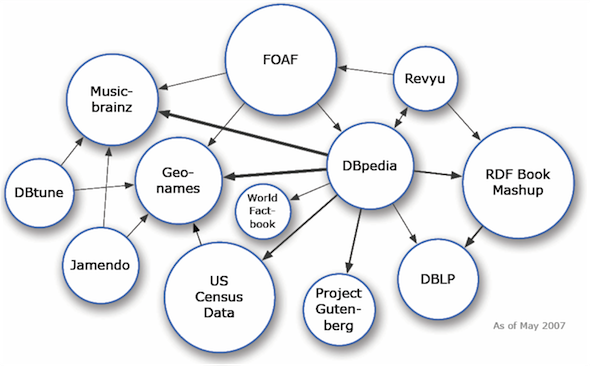
\includegraphics[width=0.9\textwidth]{img/lod-cloud2007.png}
\caption{LOD cloud as of May, 2007}
\label{fig:lodcloud2007}
\end{figure}

The Web is currently in a transition phase. After having been accessible on personal computers, it is now 
quickly moving to more and more ubiquity and entering in every part and moment of our lives. New 
devices and new ways to use them are being created. The ubiquity of the Web also creates an unseen 
abundance of information. Data is flowing onto the Web, created by users, generated by sensors, and 
stored in ever growing data farms. Geographic data is widely present on the web as they are used for location 
of Point of Interest. But this data still lack of interoperability for a better integration due to these three main factors:
\begin{itemize}
\item Vendor specific geometry support, such as Google Maps API, Yahoo Geo Technologies, etc.
\item Different vocabularies, such as W3C Basic Geo, NeoGeo, GeoSPARQL, GML XMLLiteral and vendor-specific.
\item Different spatial reference systems, such as Lambert93, WGS84, British National Grid, etc.
\end{itemize}
At the same time, many organizations are moving from legacy data stored in their databases to structured data on the web. Structured data is already present in many databases, metadata attached to medias, and in the millions of spreadsheets created everyday across the world. 


One of the key benefit of Linked Data is the use of RDF model to manipulate data on the Web, interconnect it with other data and consume it in a variety of applications. In the process of getting those datasets effectively published, there are some barriers that prevent publishers to embrace the movement, such as the following:
\begin{itemize}
\item RDF and it's different serializations is difficult to understand and use in practice compare to CSV or JSON.
\item Having a dataset, choosing a suitable vocabulary to model the data is a big challenge.
\item There are not much easy tools to guide the publishers in their process of publishing their dataset without be specialist in the different technologies: such as SPARQL, server configurations for dereferencing URIs, etc.
\item The tools for converting data into RDF are either more domain-specific, or difficult to configure for non experts.
\end{itemize}

Nevertheless, the resulting ``Web of data'' has started being populated in different domains, particularly with geospatial data, as proved by the efforts in \cite{goodwin08,linkedgeodata,deLeon2010,Salas2011}. Those efforts and initiatives follow the vision of the \textit{Semantic Geospatial Web} promotes by Max Egenhofer in \cite{egenhofer12} challenging GIS researchers to contribute to the Semantic Web effort by creating geospatial ontologies, query languages and processing techniques adapted to geospatial information on the Web. 

At the same time, the recent emergence of Linked Data radically changes the way structured data is being considered. By giving standard formats for the publication and interconnection of structured data, linked data transforms the Web into a giant database. While making data available on the Web, we need to build meaningful applications to show the value of all the huge data so that users could easily explore it, and derive new insights for it. As many information visualization tools are already present in InfoVis community\footnote{\url{http://en.wikipedia.org/wiki/Information_visualization}}, their easy adoption and usage for displaying structured data raise new challenges. Those challenges are two-folds:
\begin{itemize}
\item How to specify and define semantic web applications in terms of tools, widgets that can easily visualize RDF datasets?
\item How to mine efficiently heterogeneous structured data to derive patterns for automatically recommend the adequate visualization tool to help users building innovative applications in an affordable time.
\item How could we bridge the gap between traditional infoVis tools and Semantic Web technologies to built easily applications on top of datasets published as L(O)D?
\item How to represent and share visualizations built with datasets already present in different Open data portals, such as \texttt{data.gouv.fr} and \texttt{data.gov.uk}.  
\end{itemize}

  

\begin{figure}[ht!]
\centering{
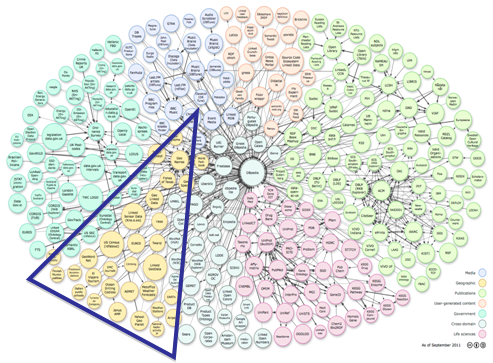
\includegraphics[scale=0.9]{img/lod-diagram-2011.png}
\caption{Linking Open Data cloud diagram 2011, by Anja Jentzsch and Richard Cyganiak. \url{http://lod-cloud.net/}}
\label{fig:lodcloud2011}
}
\end{figure}

\begin{figure}[ht!]
\centering{
\includegraphics[scale=0.1]{img/LODcloud2014.pdf}
\caption{Linking Open Data cloud diagram 2014, by Max Schmachtenberg, Christian Bizer, Anja Jentzsch and Richard Cyganiak. \url{http://lod-cloud.net/}}
\label{fig:lodcloud2014}
}
\end{figure}



\section{Research Questions}
\label{sec:questions}
 

The ubiquity of the Web is creating an unseen abundance of information. Data is flowing onto the Web, created by users, generated by sensors, and stored in ever growing data farms. Geographic data is widely present on the web as they are used for location of Point of Interest. At the same time, many organizations are moving from legacy data stored in their databases to structured data on the Web. Structured data is already present in many databases, metadata attached to medias, and in the millions of spreadsheets created everyday across the world. 
Many Linked Open Datasets have geospatial components, but still not having a common ways to describe features, spatial objects or geometries. Let us take the following three use-cases to express how challenging is to integrate geographic data from different datasets to obtain relevant answers: 
\begin{verbatim}
UC1: What DBpedia Historic Buildings are within walking distance 
     from my current location ?
UC2: What departments are located inside the bounding box 
     composed of Eurecom location and the Eiffel Tower? 
UC3: Give me the centroids of the administrative units 
     in France in Lambert93?

\end{verbatim} 
 The aforementioned use-cases take into account ``Concepts'' (e.g: Historic Building, Department) that are defined differently depending on the provider of the dataset (e.g: DBpedia, OpenStreetMap, IGN). Besides, the aforementioned use-cases implicitly make use of some specific topological functions widely used in the GIS applications, such as ``within'' , ``inside'', ``bounding box''. For example, Use Case 2 also mentioned Lambert93, a specific projection of data in France. Our aim is to contribute to the actual efforts in representing geographic objects to leverage the barrier of integration of geospatial data both by the pubishers and the lay users consuming the data. 

Our main concern is to tackle the problematic within the workflow of publication in two directions, more likely to happen at the beginning and the end: 
\begin{itemize}
\item (i) Geographic Information on the Web of data: as an application of the life-cycle of publishing geodata.
\item (ii) Visualization tools for building innovative applications consuming structured data: as for leveraging the process of creating applications on-top of semantic data to highlight some relevant knowledge to the users.

\end{itemize}

In \cite{koubarakis12}, the authors mentioned many research topics in the area of linked geospatial data. In this thesis, we try to find answers to the following challenges:

\begin{enumerate}

\item \textit{Vocabularies:} How do we model geospatial information on the Web? How do we assess geospatial ontologies? How to serialize complex geometry? 
\item \textit{Query languages:} How do we write efficient queries that target geospatial Web? How do store and index geodata in RDF ?
\item \textit{Datasets:} How do we extract and convert geodata to expose on the Web? What are the best practices for representing complex geometries on the Web? How can we integrate fully compatibility of CRSs on datasets? 
\item \textit{Publication:} How can we develop scalable frameworks for covering the workflow of publishing geodata? What are the appropriate triple stores for handling geodata? What are the metrics to use for interconnecting different geodata resources on the Web?  
\item \textit{Applications and user interfaces:} How do we generate interesting visualizations of linked geospatial data? What are appropriate high-level APIs that ease the development of user interfaces for geospatial data? Can we rely on existing map platforms such as Google Maps, Bing Maps or OpenSteetMap?
\end{enumerate}

In this thesis we mainly focus on the first, third, fourth and fifth of the above topics, and acknowledge existing efforts on the rest of the topic. We tackle the issues and challenges both from publishers and users point of view. The publishers need pragmatic solutions that help to choose a vocabulary, find a tool to convert ShapeFiles according to well-known vocabularies, then generate and publish the data following some best practices.


After the publication of the dataset using LD paradigm, the logical question is: ``What next''? Publishers need to be able to understand their dataset; while developers have to build application out of the datasets. It is clear there is a huge amount of structured data on the Web, with the expectation to have more and more 
data to be published as LOD. This huge amount of "structured big data" fails to reach the non-expert users 
so far, due to the complexity of different technologies used to model and query the data. Thus, it is 
important to create ``visual applications'' on top of the generated datasets to explore, analyze and showcase 
some of the potential of linked data to non-expert users. In this process, some challenging research questions have to be addressed, such as the following:

\begin{itemize}
\item  How to find the suitable visualization according to the datasets without showing the complexity of SPARLQ queries?
 \item  What are the important properties to visualize for entities, depending on the domain and the users' expectations?
 \item  How to bridge the gap between existing traditional tools of Information Visualization, mostly using CSV/XLS, JSON or proprietary formats to easily integrate RDF models as input?
 \item How to make interoperable applications built on top of Government Open Data catalogues? How to reuse existing applications?
\end{itemize}
 
 While trying to answer to the aforementioned challenges, we are aware of some existing approaches dealing with visualizations for Linked Data. 


\section{Contributions}
\label{sec:contributions}
In this section, we provide the main contributions organized in three main sections of our thesis: model and publication of geospatial data, visualizations of data and applications on the Web and contribution to standards. 

\subsection{Modeling, publishing and querying geodata}
The need for geolocation is crucial for many applications for both human and software agents. More and more data is opened and interlinked using Linked Data principles, and it is worth modeling geographic data efficiently by reusing as much as possible from existing ontologies or vocabularies that describe both the geospatial features and their shapes. In the first part of our work, we survey different modeling approaches used by the Geographic Information System (GIS) and the Linked Open Data (LOD) communities. Our aim is to contribute to the actual efforts in representing geographic objects with attributes such as location, points of interest (POI), and addresses on the web of data. We focus on the French territory and we provide examples of representative vocabularies that can be used for describing geographic objects. We propose some alignments between various vocabularies (DBpedia, GeoNames, Schema.org, LinkedGeoData, Foursquare, etc.) in order to enable interoperability while interconnecting French geodata with other datasets. 

Regarding this aspect of our research, we have achieved the following tasks:
 \begin{itemize}
  \item We have proposed an ontology describing features and point of interest for the French territory, by reusing existing taxonomy (GeOnto) and aligning it to other related vocabularies of the domain.
  \item  We studied how to extend the existing vocabularies for geographic domain to take into account efficient modeling for complex geometries. By doing so, tackle the complex geometry representation issues in the Web of Data, describing the state of implementations of geo-spatial functions in triple stores and comparing them to the new GeoSPARQL standard.  We finally make some recommendations and advocate for the reuse of more structured vocabulary for publishing topographic entities to better address the IGN-France requirements.
  
 \item We have made a comparative study of the triple stores, comparing their capability to store spatial information and their implementation of topological functions with respect to the ones 
existing in OGC\footnote{\url{http://www.opengeospatial.org/}} standards.
 \item  We have designed and implemented vocabularies for describing complex geometries with different coordinate systems, with direct application to the French administrative units.
 
 \item We have interlinked French Authoritative geodata resources with existing datasets, such as LinkedGeodata, GADM, NUTS and Geonames.
 
 \item We have contributed to the creation of a French LOD Cloud by publishing many datasets as LOD covering the French territory.
 

\end{itemize}

 
%\subsection{Modeling Geographic Information in LOD} \label{model}
%In France, there is  currently a joint effort to publish geographic information in RDF (Resource Description Framework) and interlink them with relevant datasets. GeOnto is an ontology describing geospatial features for the French territory. We have proposed to align GeOnto with other popular vocabularies in the geospatial domain, using Silk for schema mapping and we have evaluated the results.

\subsection{Visualization Tools in Linked Government Data} \label{visu}

We first review some innovative applications that have been developed on top of datasets that have been opened by governments (UK, USA, France) and local authorities. We have then derived and proposed some use cases (8 UCs) that can be developed to consume data from the different main providers in the French level: INSEE, DILA, IGN, FING, etc. We mention that the most interesting UCs are the ones which show the added value of having interconnected datasets. These UCs,  developed and deployed, can be useful to show the benefits of Linked Data in a variety of domains such as Education, Tourism, Cultural Heritage, Civil administrations, Judicial Court, Medicine, etc. 

Regarding tools used for visualization, we have identified and classified them in two categories, providing for each of them relevant examples: (i)-tools that operate over RDF data, (ii) and tools that operate over other structured format. We then provide some basic criteria for assessing a given visualization tool, with some weight attached to each of the criterion. 

Moreover, regarding visualizations on top of datasets, we have contributed in this thesis by:
\begin{itemize}
\item Building an application of the French first round elections in 2012 using data from the \texttt{data.gouv.fr} and other public institutions. The application available at \url{http://www.eurecom.fr/~atemezin/DemoElection/}  built with Exhibit Framework \cite{exhibit2007} aim at showcasing the reconciliation of heterogeneous datasets: political results in CSV, unemployment rate, data of candidates, departments of France and more data from DBpedia. The user can filter by candidate image, unemployment rate and department to see the scores, with more information about the department if needed.
 
\item Implementing a generic tool for exploring geodata on a map, based on the automatic detecting of SPARQL endpoints in the LOD cloud containing geospatial datasets. 

\item Implementing an application consuming geodata and statistics combining multiple datasets in education from \url{http://data.gouv.fr} portal.

\item Building an application for conference events (confomaton) with their associated media reconciled from many social platform (instagram, twitter, etc.).

\item Building a vocabulary for structuring applications on the Web of data. The vocabulary can be used for discovering libraries or charts used to build applications. 

\item Implementing a generic plugin for annotating applications developed for contests to be included in any web page, leveraging  the generation of structured content out of webpages using the vocabulary. 


\item Implementing a wizard that analyses an RDF dataset and recommend visualization based on predefined categories, using generic SPARQL queries for easing the exploration of datasets published as LOD. 


\end{itemize}

\subsection{Contributions to Standards}
We contributed to the W3C Government Linked Data Working Group (GLD WG)\footnote{http://www.w3.org/2011/gld/} activity from July, 2011 until December, 2013.  The objective of the Working Group was to \textit{``provide standards and other information which help governments around the world publish their data as effective and usable Linked Data using Semantic Web technologies''}.

The group had three main task forces:
\begin{itemize}
\item \textbf{Task Force \#1} aims to create a linked data community directory\footnote{http://dir.w3.org} and to maintain it on-line about deployments, vendors, contractors, end-user applications. In this work, we contribute to define the requirements and providing data for the French organizations in the directory.

\item \textbf{Task Force \#2} aims at providing \textbf{``Best Practices''} for Publishing Linked Data by producing recommendations regarding vocabulary selection, URI construction, Linked Data Cookbook, versioning, stability and provenance. Here, we have prepared a check- list to help government to select and re-use vocabularies in their project. We have also proposed our vision of the Linked Open Data Life cycle, best practices for creating URIs. We were editor for the Linked Data Glossary \cite{glossairegld} published as Note document. Apart from contributing in many sections of the document ``Best Practices for Publishing Linked Data'' \cite{bpgld}.

\item \textbf{Task Force \#3} goal was to provide relevant vocabularies to be used by governments or local authorities in their process of exposing their data. We have participated actively in the discussions on the different vocabularies published as recommendations by the W3C such as Data Cube \cite{dcube}, ORG vocabulary \cite{org} and DCAT \cite{dcat} vocabulary.
\end{itemize}

Regarding the use of standard vocabularies we have contributed on : 
\begin{itemize}

\item  Proposing a method to harmonize prefixes on the web of data  with two services: Linked Open Vocabularies (LOV)\footnote{\url{http://lov.okfn.org/dataset/lov/}} and prefix.cc\footnote{\url{http://prefix.cc}}. The former is currently a maintained hub of curated vocabularies on the Web, while the latter is a focal point for developer to register and look-up prefixes for their resources or ontologies. The approach proposed can be extended to any catalogue of vocabulary as long as the vocabularies fulfill the requirements to be inserted into LOV catalogue. 

\item  Designing and implementing a new method for ranking vocabularies based on the computation of Information Content (IC) and Partitioned Information Content (PIC) metrics.

\item We have developed a tool than answer in real-time whether different licenses present in the dataset and vocabularies are either compatible or not. 
\end{itemize}

\section{Thesis Outline}
\label{sec:thesis-structure}

The work presented within this thesis is composed of three major parts. The remainder of the thesis proceeds as follows:

\begin{itemize}
\item In the first part of this thesis, we focus on the various models/vocabs for representing geography/geometry. We survey the state of the triple stores and describe particular problems (coordinate systems, etc.) and highlight our contributions: new vocabularies, an online converter between CRS, etc. We also describe how geography database can then be converted into RDF using the Datalift process. We then show how those datasets can be interlinked (possibly trying different instance matching tools) and it will conclude with a thorough analysis of those alignments in the case of the IGN-France datasets. More specifically:

 \begin{itemize}
  \item \textbf{Chapter \ref{ch:ch1}} describes the current limitations of geodata on the Web and the different vocabularies we propose for geometries, coordinate reference systems and feature  types. We also propose  some best practices to publish geodata on the web.
  \item \textbf{Chapter \ref{ch:ch2}} focuses on tools for publishing and querying geodata, their differences and applications. We describe Datalift platform, an open source platform to lift raw data sources to semantic interlinked data sources. After comparing Datalift with the Geoknow stack, we apply it in the process of publishing French Administrative Units and French Gazetteer datasets. We then presents the status of the \textit{French LOD}(\textit{FrLOD}) cloud and some sample of queries over structured geometries published within \texttt{data.ign.fr} endpoint. 
 \end{itemize}

%\item 
 \item In the second part of the thesis, we cover three main issues regarding how to present RDF to end-users. First, we make a state of the art review of existing tools and solutions for visual representation and exploration of RDF (Visualbox, LODSpeaKr, Map4RDF, Linked Data Visualization Model,etc.) Then, we present our contribution: the wizard for visualizations including the vocabulary for describing visualizations, the prototype itself, etc. Third, we present two applications applied to events and statistics to showcase the consumption of interlinked datasets in a new fashion. Then, we present a mechanism of extracting and reusing application in open data events. Finally, we provide some insights on revealing the ``important'' properties of Entities for visualization by reverse engineering the Google Knowledge Panel (GKP). This part is divided in two chapters:
 \begin{itemize}
 \item \textbf{Chapter \ref{ch:ch4}} provides a survey on visualozation tools and applications, with their limitations. We also describe the status of the applications on the web and provide a classification of so-called ``Linked Data Applications''.
 \item  In \textbf{Chapter \ref{ch:ch5}}, we present our contribution on new approaches to generate visualizations ans applications. We first propose a novel approach for category-based visualizations. We then show an application for geographic domain. Two applications related to events and statistics are also described. Finally, we propose how to improve the discovery of applications contests in Open Data events, through a model and a universal plugin for RDF population. 
 \end{itemize}
 \item In the last part of the thesis in \textbf{Chapter \ref{ch:ch6}}, we describe various contributions on the Linked Open Vocabularies (catalog description, vocabulary publications, APIs and endpoints): prefixes harmonization, vocabulary ranking metrics using information content. We also present some insights on checking licenses compatibility between vocabularies and datasets with the defeasible deontic logic by creating an automatic tool for licenses checking. 
\end{itemize}

 In \textbf{Chapter \ref{ch:conc}}, we conclude about the presented works, highlight its limitations and suggest new research directions.